\graphicspath{{./images/}}

\chapter{Kontextabgrenzung}

\section{Fachlicher Kontext}
\textcolor{red}{/* TODO hier abgebildet ist der Workflow, Grafik anpassen mit einer Box Kunde füllt Vertragsformular aus */}
\begin{center}
	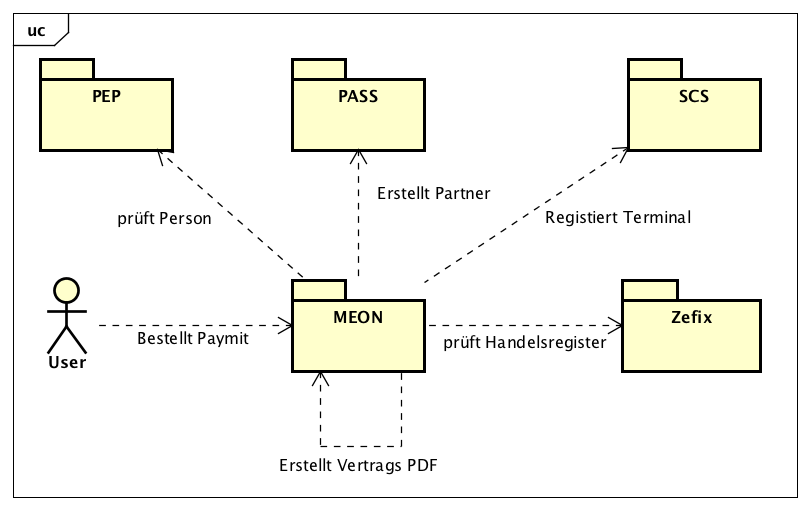
\includegraphics[scale=0.7]{kontext.png}
\end{center}


\section{Technischer Kontext}

Die Applikation MEON basiert auf Spring Boot für den Onboarding Server, AngularJS als Frontend sowie Camunda als Workflow Engine. Die Anwendung wird mittels der Container Technologie Docker auf der OpenShift Plattform ausgerollt. 

\section{Externe Schnittstellen}

\subsection{PASS Schnittstelle}
		
\subsubsection{Identifikation}

REST Schnittstelle (URL)

\subsubsection{Bereitgestellte Resourcen}

\begin{itemize}
 \item Anlegen eines neuen Partners
 \item Unblock des Kontos, damit der Partner Zahlungen ausbezahlt bekommt
\end{itemize}

\subsubsection{Fehlerszenarien}

\begin{itemize}
 \item Schnittstelle nicht verfügbar
 \item invalide Daten
\end{itemize}
Bei einem Fehler bleibt der Request im Workflow stehen. Bei einem technischen Fehler wird periodisch versucht den Request nochmals zu schicken. Bei einem Datenqualitätsfehler muss der Datensatz im Workflow korrigiert werden.

\subsubsection{Variabilitität und Konfigurierbarkeit}

Der Partner wird anhand eines hinterlegten Templates erstellt, nur die davon unterschiedlichen Felder müssen geliefert werden. Die Konfigurierbarkeit ist entsprechend in dem Template, für welches die Referenz über die Schnittstelle mitgegeben wird. Die Schnittstelle ist versioniert..
Die URL zeigt auf eine VIP (Virtual IP). D.h. bei einem Ausfall wird (manuell) der Loadbalancer auf den Ausfallserver gerichtet. Da muss die Applikation ebenfalls laufen.

\subsubsection{Qualitätseigenschaften}

Hochverfügbar da über zwei Datenzentren mittels Hot Cold gesichert.
Die Schnittstelle nimmt nur zwischen 07:00 und 19:00 Requests an (tagfertige Verarbeitung).
	
\subsubsection{Entwurfsentscheidungen} 

Die Annahme der Request zwischen 7 und 19 Uhr basiert auf dem Modifizerungsmodus für die Benutzer. Theoretisch könnten auch ausserhalb dieser Zeiten neue Partner erstellt werden, da sie das laufende Business nicht beeinflussen. Modifikationen hingegen müssen auf diesen Modus schauen.

\subsubsection{Benutzungshinweise} 

User muss im PASS angelegt sein und die entsprechende Security Role für die Institution beistzen (ist ein technischer, aber auch ein normaler User könnte mit den Berechtigungen das Interface bedienen).
Der Service liegt in der PCI Zone und kann aus der PubDMZ nicht angesprochen werden
	
\subsection{SCS Schnittstelle}

\subsubsection{Identifikation}

\subsubsection{Bereitgestellte Resourcen}

\subsubsection{Fehlerszenarien}

\begin{itemize}
	\item Schnittstelle nicht verfügbar
	\item invalide Daten
\end{itemize}
Im Fehlerfall bleibt der Request im Workflow stehen. Ist es ein technischer Fehler wird periodisch versucht den Request zu schicken, im Fall von falschen Daten muss der Datensatz im Workflow korrigiert werden.

\subsubsection{Variabilitität und Konfigurierbarkeit}

\subsubsection{Qualitätseigenschaften}

\subsubsection{Entwurfsentscheidungen} 

\subsubsection{Benutzungshinweise} 

\subsection{UID Schnittstelle}

\subsubsection{Identifikation}
URL

\subsubsection{Bereitgestellte Resourcen}
Unternehmensdaten abfragen

\subsubsection{Fehlerszenarien}
\begin{itemize}
	\item Service nicht verfügbar --> Der User muss von Hand die Daten in der Webapplikation erfassen
	\item Invalide Daten 
\end{itemize}



\subsubsection{Variabilitität und Konfigurierbarkeit}
Histerix

\subsubsection{Qualitätseigenschaften}

\subsubsection{Entwurfsentscheidungen} 

\subsubsection{Benutzungshinweise} 

\subsection{ZEFIX Schnittstelle}

\subsubsection{Identifikation}
URL
\subsubsection{Bereitgestellte Resourcen}
Abfrage Handelsregisterauszug

\subsubsection{Fehlerszenarien}
\begin{itemize}
	\item Unternehmen nicht vorhanden
	\item Service nicht verfügbar
\end{itemize}
In beiden Fällen muss der Handelsregisterauszug manuell hochgeladen werden.

\subsubsection{Variabilitität und Konfigurierbarkeit}
Kantone haben unterschiedliche Zugangsurls und Provider
Histerix

\subsubsection{Qualitätseigenschaften}

\subsubsection{Entwurfsentscheidungen} 

\subsubsection{Benutzungshinweise} 

\subsection{Adressen Schnittstelle}

\subsubsection{Identifikation}
URL

\subsubsection{Bereitgestellte Resourcen}
Abfrage Plz/Ort und Strasse

\subsubsection{Fehlerszenarien}
Falls der Service nicht verfügbar ist muss der User die Adresse ohne Autofill ausfüllen.

\subsubsection{Variabilitität und Konfigurierbarkeit}
Histerix

\subsubsection{Qualitätseigenschaften}

\subsubsection{Entwurfsentscheidungen} 

\subsubsection{Benutzungshinweise} 


